% File Vault - reviewer-facing product, implementation, and delivery document
% Compile with: pdflatex hiring-task-documentation.tex (run twice for references).
\documentclass[11pt,a4paper]{article}
\usepackage[margin=0.82in,headheight=15pt]{geometry}
\usepackage[utf8]{inputenc}\usepackage[T1]{fontenc}\usepackage{textcomp}\usepackage{lmodern}\usepackage{microtype}
\usepackage{booktabs}\usepackage{tabularx}\usepackage{longtable}\usepackage{array}
\usepackage{enumitem}\usepackage{xcolor}\usepackage{listings}\usepackage{tcolorbox}\usepackage{tikz}\usepackage{graphicx}
\tcbuselibrary{skins}
\usetikzlibrary{arrows.meta,positioning,fit,calc}
\usepackage{titlesec}\usepackage{fancyhdr}\usepackage{float}\usepackage{hyperref}

\definecolor{navy}{HTML}{080A25}\definecolor{ink}{HTML}{101D35}\definecolor{indigo}{HTML}{4354D8}
\definecolor{cyan}{HTML}{54D8E5}\definecolor{muted}{HTML}{71809A}\definecolor{wash}{HTML}{F4F6FB}
\definecolor{line}{HTML}{DEE5F0}\definecolor{success}{HTML}{197B78}
\definecolor{violet}{HTML}{B84DFF}\definecolor{coral}{HTML}{FF6B7A}\definecolor{gold}{HTML}{FFC857}
\definecolor{mint}{HTML}{DDF8F1}\definecolor{lavender}{HTML}{EEE8FF}\definecolor{peach}{HTML}{FFF0E6}
\hypersetup{colorlinks=true,linkcolor=indigo,urlcolor=indigo,pdftitle={File Vault - Product, Architecture, and Delivery Documentation},pdfauthor={Engineering}}
\setlength{\parindent}{0pt}\setlength{\parskip}{6pt}
\setlist[itemize]{leftmargin=1.4em,itemsep=2pt,topsep=3pt}\setlist[enumerate]{leftmargin=1.6em,itemsep=3pt,topsep=3pt}
\newcolumntype{Y}{>{\raggedright\arraybackslash}X}\newcolumntype{P}[1]{>{\raggedright\arraybackslash}p{#1}}
\pagestyle{fancy}\fancyhf{}\fancyhead[L]{\color{indigo}\small\textbf{FILE VAULT} \;|\; ENGINEERING DOCUMENTATION}\fancyfoot[C]{\color{muted}\small\thepage}
\renewcommand{\headrulewidth}{0.4pt}\renewcommand{\footrulewidth}{0pt}
\titleformat{\section}{\Large\bfseries\color{indigo}}{\thesection}{0.7em}{}\titleformat{\subsection}{\large\bfseries\color{ink}}{\thesubsection}{0.7em}{}\titleformat{\subsubsection}{\normalsize\bfseries\color{indigo}}{\thesubsubsection}{0.7em}{}
\titlespacing*{\section}{0pt}{22pt}{8pt}\titlespacing*{\subsection}{0pt}{14pt}{5pt}
\lstset{basicstyle=\ttfamily\small,breaklines=true,columns=fullflexible,backgroundcolor=\color{wash},frame=single,rulecolor=\color{line},framerule=0.4pt,showstringspaces=false}
\newcommand{\status}[1]{\textcolor{success}{\textbf{#1}}}\newcommand{\code}[1]{\texttt{\small #1}}
\newcommand{\featurebadge}[2]{\fcolorbox{#1}{wash}{\textcolor{#1}{\textbf{\small #2}}}}
\graphicspath{{screenshots/}}
\newcommand{\shot}[3]{\begin{figure}[H]\centering\includegraphics[width=0.91\textwidth,height=3.25in,keepaspectratio]{#2}\caption{#1}\label{fig:#3}\end{figure}}

\begin{document}
\begin{titlepage}\thispagestyle{empty}\vspace*{0.7in}\begin{center}
{\Large\textcolor{indigo}{\textbf{FILE VAULT}}}\par\vspace{0.22in}
{\fontsize{31}{36}\selectfont\textcolor{navy}{\textbf{Product, Architecture,\\[2pt] and Delivery Documentation}}}\par\vspace{0.22in}
{\large\textcolor{muted}{A private workspace for storing, organizing, and sharing files}}\par\vspace{0.55in}
\fcolorbox{line}{wash}{\parbox{0.82\textwidth}{\centering\small\color{ink}File Vault gives each user a private place to upload, organize, search, share, preview, and download files. It records who owns each file, stores identical content once, enforces quotas and rate limits, and gives administrators a separate oversight view.}}
\end{center}\vfill
\begin{tabularx}{\textwidth}{P{0.26\textwidth}Y}\toprule
\midrule\textbf{Application} & File Vault --- a secure file storage and sharing system.\\
\textbf{Technology} & Go REST API, React and TypeScript frontend, PostgreSQL, Redis, Docker, Kubernetes, Helm, and GitHub Actions.\\
\bottomrule\end{tabularx}\vspace{0.25in}\end{titlepage}
\tableofcontents\newpage

\begin{tcolorbox}[enhanced,colback=peach,colframe=coral,boxrule=0.7pt,arc=5pt,left=10pt,right=10pt,top=7pt,bottom=7pt]
\textcolor{coral}{\textbf{How to read this document:}} Core features establish product behavior; deliverables point to the submitted artifacts; bonus points identify work beyond the mandatory path. Each item states the implementation and the evidence location.
\end{tcolorbox}

\section{Product overview}
\subsection{What the product is about}
File Vault is a private file workspace for individuals and teams. Each registered user gets a vault for uploading one or many files, organizing them into folders, finding them with search and filters, checking metadata, previewing supported formats, downloading content, and managing access. Ownership is explicit: the uploader controls deletion and sharing. Administrators can review workspace activity, but they cannot delete files owned by another user.

The implementation also covers the details that matter in a file service. SHA-256 content addressing stores identical content once. Quota usage is based on each user's logical files. Storage savings come from the difference between logical file sizes and the physical blobs actually stored. Public downloads are counted and shown in analytics.

\subsection{Primary user journeys}
\begin{itemize}
\item A new user registers, signs in, and receives a private vault with the default quota.
\item A user uploads files through the picker or drag-and-drop. Each file is streamed, validated, hashed, quota-checked, and either stored as a new blob or linked to an existing blob.
\item A user views a file list, opens metadata, moves files into folders, previews supported files, downloads content, and deletes only files they own.
\item A user shares a file or folder directly with another registered user or creates a public link, and can later revoke access.
\item An administrator uploads and shares files, lists all workspace files with uploader details, and views protected usage, download, and deduplication statistics.
\end{itemize}
\subsection{Product architecture at a glance}
\begin{center}
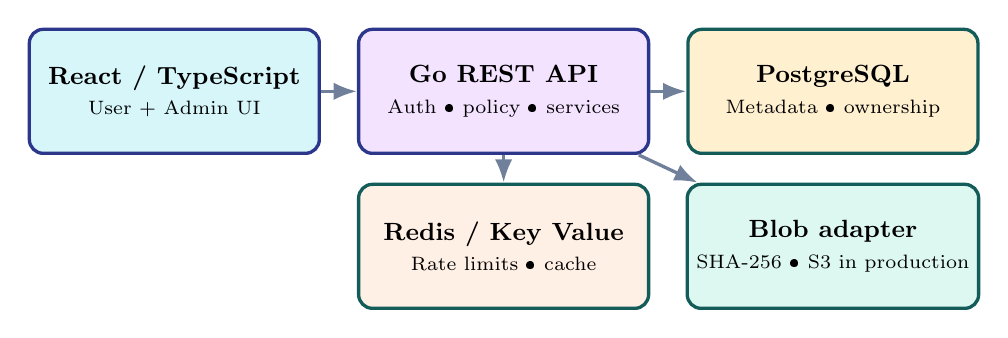
\begin{tikzpicture}[node distance=10pt and 13pt,svc/.style={rounded corners=5pt,draw=indigo!65!black,very thick,minimum width=1.45in,minimum height=0.62in,align=center,font=\small\bfseries},store/.style={rounded corners=5pt,draw=success!75!black,very thick,minimum width=1.45in,minimum height=0.62in,align=center,font=\small\bfseries},arr/.style={-Latex,very thick,draw=muted}]
\node[svc,fill=cyan!24] (ui) {React / TypeScript\\\normalfont\scriptsize User + Admin UI};
\node[svc,fill=violet!16,right=of ui] (api) {Go REST API\\\normalfont\scriptsize Auth \textbullet\ policy \textbullet\ services};
\node[store,fill=gold!28,right=of api] (db) {PostgreSQL\\\normalfont\scriptsize Metadata \textbullet\ ownership};
\node[store,fill=mint,below=of db] (blob) {Blob adapter\\\normalfont\scriptsize SHA-256 \textbullet\ S3 in production};
\node[store,fill=peach,below=of api] (redis) {Redis / Key Value\\\normalfont\scriptsize Rate limits \textbullet\ cache};
\draw[arr] (ui) -- (api);
\draw[arr] (api) -- (db);
\draw[arr] (api) -- (blob);
\draw[arr] (api) -- (redis);
\end{tikzpicture}
\end{center}
\begin{center}\textcolor{muted}{\scriptsize The diagram separates the UI, API, database, blob storage, and shared runtime services.}\end{center}
\shot{Product overview}{product-overview.png}{product-overview}

\section{Technology stack}
\begin{tabularx}{\textwidth}{P{0.22\textwidth}Y Y}\toprule\textbf{Layer}&\textbf{Technology}&\textbf{How it is used}\\\midrule
Backend&Go&Modular monolith with typed handlers, services, policies, health checks, and structured logging.\\
API&REST over HTTP&Authentication, uploads, file management, folders, sharing, content, search, statistics, events, and administration.\\
Frontend&React + TypeScript + Vite&Responsive vault UI, authentication, upload/drop interaction, filters, file details, sharing, folders, admin tabs, and charts.\\
Database&PostgreSQL&Users, sessions, files, blobs, folders, tags, shares, downloads, audit events, migrations, and indexes.\\
Cache/limits&Redis&Shared rate-limiter state for multi-replica deployments; local fallback for evaluation.\\
Blob storage&S3-compatible adapter in production; local adapter for development&Content-addressed blobs use shared object storage in production and local disk only for local Compose.\\
Visualization&Recharts&Responsive user and administrator storage, deduplication, quota, and activity visualizations.\\
Testing&Go test, vet, race detector, Playwright&Unit, integration, authorization, upload, MIME, deduplication, UAT, and smoke verification.\\
Delivery&Docker, Kubernetes, Helm, GitHub Actions&Reproducible containers, deployment manifests, charts, CI checks, and image builds.\\\bottomrule\end{tabularx}

\section{Project setup}
\subsection{Run the complete stack}
The quickest local setup uses Docker Desktop. Start the Docker engine, copy the example environment file, and bring up the services:
\begin{lstlisting}[language=bash]
Copy-Item .env.example .env
docker compose up --build -d
docker compose ps
\end{lstlisting}
Open \code{http://localhost:5173}. Compose starts PostgreSQL, Redis, the Go API, and the Nginx frontend. The API applies database migrations during startup. The local administrator seed is optional and reads its credentials from runtime environment variables; the local evaluation values are documented in \code{docs/seed-data.md}.

\subsection{Run the services separately}
For backend work, start PostgreSQL and Redis first, set \code{DATABASE\_URL} and \code{REDIS\_URL}, then run the API from \code{backend/}. For frontend work, install dependencies and start Vite from \code{frontend/}:
\begin{lstlisting}[language=bash]
# terminal 1
cd backend
go run ./cmd/api

# terminal 2
cd frontend
npm ci
npm run dev
\end{lstlisting}
The frontend development server proxies API requests according to its local configuration. Use the Compose path when you need the same proxy, storage, and dependency layout as the full application.

\subsection{Verify the setup}
After the services are healthy, run the repository checks:
\begin{lstlisting}[language=powershell]
.\scripts\verify.ps1
.\scripts\core-smoke.ps1
\end{lstlisting}
The checks cover formatting, \code{go vet}, backend tests, frontend linting and build checks, Docker image validation, and the core application smoke flow. The deployment guide in \code{docs/deployment.md} covers Kubernetes, Helm, and Render configuration.

\section{Core features and implementation}
The following sections map the hiring-task requirements to the implementation.

\subsection{File uploads}
\textbf{Requirement.} Support single and multiple file uploads, drag-and-drop upload in the frontend, and content validation against the declared MIME type.

\textbf{Implementation.} The frontend accepts multiple files and handles drops anywhere in the vault without letting the browser navigate away. The upload service streams each multipart file, applies request and per-file limits, calculates its SHA-256 digest, and checks the content against the declared MIME type. Each file gets its own result, so a mixed batch can report successes and rejections separately. The service rejects forged extensions and mismatched content before it commits anything.
\shot{Upload and drag-and-drop}{upload-drag-drop.png}{upload-drag-drop}

\subsection{File management and sharing}
\textbf{Requirement.} Users can list and view owned files with detailed metadata; organize files into folders; share files and folders publicly or keep them private; share directly with specific users; show public download counters; and allow only the uploader to delete a file.

\textbf{Implementation.} File metadata belongs to an owner and includes uploader identity, logical size, detected and declared MIME types, upload time, blob size, reference count, visibility, and download count. Folders belong to an owner and can have a parent folder. Files can move between the root and folders. A folder's context menu provides open, rename, share, and delete actions, both on the home inventory and in the folders view.

Public links use random tokens; the database stores only their hashes. Direct shares store the recipient and permission, inherit folder access for files inside a shared folder, and support revocation. Files and folders are private by default. Delete handlers enforce ownership, protect other users' files, and remove a physical blob only after its final logical reference is gone.
\shot{File details and sharing}{file-details-sharing.png}{file-details-sharing}

\subsection{Search and filtering}
\textbf{Requirement.} Search by filename; filter by MIME type, size range, date range, tags, and uploader name; combine filters; optimize queries for scale.

\textbf{Implementation.} The list endpoint accepts parameterized filters and bounded cursor pagination. Filename search uses PostgreSQL text search with index support. Owner, uploader, folder, upload date, MIME, size, and tag conditions are combined in one query. The frontend exposes the requested categories: MIME type, minimum and maximum bytes, uploaded-after and uploaded-before dates, tag, uploader name, and filename search. The two date fields are the inclusive upload-time range. The backend converts them to UTC boundaries and rejects an end date before a start date. Search-plan evidence is in \code{docs/performance/search-plan.md}.
\shot{Search and filtering}{search-filtering.png}{search-filtering}

\subsection{Rate limiting and quotas}
\textbf{Requirement.} Enforce per-user API rate limits with a configurable default of 2 calls per second, configurable per-user storage quota with a default of 10 MB, and proper error codes/messages.

\textbf{Implementation.} The limiter uses the authenticated user ID as its key. \code{API\_RATE\_PER\_SECOND} sets the rate and \code{API\_RATE\_BURST} sets the allowed burst. \code{USER\_QUOTA\_BYTES} sets the storage quota and defaults to 10 MiB (10\,485\,760 bytes). Uploads check the quota transactionally against logical owned bytes, while duplicate content is not stored twice physically. The API returns structured errors: HTTP 429 for rate limits and HTTP 413 with a quota-specific code when storage is full. When \code{REDIS\_URL} is configured, replicas share limiter state through Redis.

\subsection{Storage statistics}
\textbf{Requirement.} Display total deduplicated storage used, original usage without deduplication, and savings in bytes and percentage.

\textbf{Implementation.} Original usage is the sum of the active logical file sizes owned by the user. Deduplicated usage is the sum of distinct referenced blob sizes. Savings equal original usage minus deduplicated usage; the percentage divides those savings by original usage and safely handles zero. The user dashboard shows summary cards and charts. Administrators see workspace totals, download counts, user and file counts, and the same storage calculations at workspace scope.
\shot{Storage statistics}{storage-statistics.png}{storage-statistics}

\subsection{Admin panel}
\textbf{Requirement.} Admins can upload files and share them with other users; the admin panel lists all files with uploader details; admins can view download counts and usage statistics.

\textbf{Implementation.} Role checks protect every administrator route. The administrator area separates upload/share actions, an all-files inventory with uploader name and email, MIME type, size, date, and download count, and a Statistics tab with workspace usage and Recharts charts. Administrators can inspect and share files, but cannot delete files owned by another user. User and administrator views use the same logical and physical storage definitions, with different scopes.
\textbf{Local evaluation access.} The seeded administrator account uses email \code{admin@example.com} and password \code{AdminVault!2026}. This credential is configured only for local evaluation and must be replaced before a shared or production deployment.
\shot{Administrator oversight}{admin-oversight.png}{admin-oversight}

\section{Deliverables}
\begin{tcolorbox}[enhanced,colback=gold!13,colframe=gold!70!black,boxrule=0.8pt,arc=5pt,left=10pt,right=10pt,top=7pt,bottom=7pt]
\featurebadge{gold!70!black}{SUBMISSION ARTIFACTS}\quad\textbf{Deliverables}\quad\small The table maps each deliverable to the code or artifact that provides it.
\end{tcolorbox}
\begin{longtable}{P{0.25\textwidth}P{0.17\textwidth}P{0.48\textwidth}}\toprule\textbf{Deliverable}&\textbf{Status}&\textbf{How it is delivered}\\\midrule
Go backend&\status{Complete}&\code{backend/} contains API server, domain services, handlers, policies, health endpoints, configuration, logging, and tests.\\
REST or GraphQL API&\status{Complete}&REST is the shipped runtime; a GraphQL SDL contract is retained because the brief accepts REST and prefers GraphQL.\\
PostgreSQL schema/migrations&\status{Complete}&Forward-only migrations define users, auth sessions, blobs, files, folders, tags, shares, downloads, audit events, indexes, and constraints.\\
React/TypeScript frontend&\status{Complete}&\code{frontend/} provides authenticated vault, folders, upload/drop UX, details, sharing, filtering, admin navigation, and analytics.\\
Docker Compose&\status{Complete}&Compose runs PostgreSQL, Redis, API, and Nginx frontend with health checks and persistent local volumes.\\
Documentation&\status{Complete}&Contracts, database/storage notes, UAT checklist, delivery matrix, deployment guide, AI methodology, and this report are maintained under \code{docs/}.\\\bottomrule\end{longtable}

\section{Product orchestration and infrastructure}
\subsection{Runtime orchestration}
Docker Compose runs PostgreSQL for relational data, Redis for shared limit state, the Go API for business logic, and Nginx for the React build and API/public-content proxying. Health checks wait for dependencies before the API starts. The API runs seed logic only when runtime seed variables are supplied. Production secrets and passwords stay out of source control.

\subsection{Upload and deduplication flow}
\begin{center}
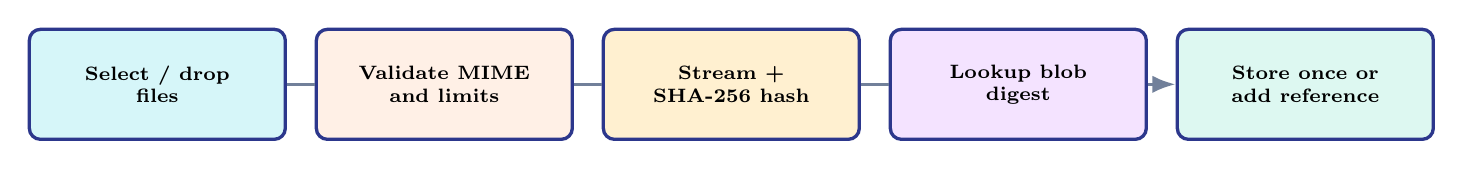
\begin{tikzpicture}[node distance=8pt and 10pt,flow/.style={rounded corners=4pt,draw=indigo!65!black,very thick,minimum width=1.28in,minimum height=0.55in,align=center,font=\scriptsize\bfseries}, every path/.style={-Latex,very thick,draw=muted}]
\node[flow,fill=cyan!24] (select) {Select / drop\\files};
\node[flow,fill=peach,right=of select] (validate) {Validate MIME\\and limits};
\node[flow,fill=gold!28,right=of validate] (hash) {Stream +\\SHA-256 hash};
\node[flow,fill=violet!16,right=of hash] (lookup) {Lookup blob\\digest};
\node[flow,fill=mint,right=of lookup] (link) {Store once or\\add reference};
\draw (select) -- (validate) -- (hash) -- (lookup) -- (link);
\end{tikzpicture}
\end{center}
\begin{center}\textcolor{muted}{\scriptsize Logical file rows preserve ownership and history; one physical blob may serve many references.}\end{center}

\subsection{Data and storage orchestration}
The database owns logical metadata and relationships. The blob adapter owns physical content. Each file row points to a content-addressed blob by digest, and several file rows can point to the same blob. Transactions update reference counts. Deletion removes the physical object only after the last reference disappears. Production uses the S3-compatible adapter so all API replicas share the same content store.

\subsection{Security orchestration}
Authentication uses Argon2id password hashes, database-backed sessions, HttpOnly cookies, CSRF tokens, and explicit owner/admin checks. Public share tokens are random, and only their hashes are stored. Private, direct-share, and public-content paths have separate authorization checks. The API returns structured error codes without exposing internal details.

\subsection{Deployment orchestration}
Raw Kubernetes manifests live in \code{k8s/}; the Helm chart lives in \code{helm/balkanid/}. They define API and frontend Deployments and Services, PostgreSQL, Ingress, ConfigMap, a Secret template, probes, a service account, and PVCs. A cloud launch should use managed PostgreSQL and Redis, shared object storage, TLS, external secrets, backups, and monitoring.

\section{Bonus points implemented}
\begin{tcolorbox}[enhanced,colback=violet!9,colframe=violet!75!black,boxrule=0.8pt,arc=5pt,left=10pt,right=10pt,top=7pt,bottom=7pt]
\featurebadge{violet!75!black}{BEYOND THE CORE}\quad\textbf{Bonus coverage}\quad\small These items extend the mandatory product into deployment, scale, automation, and reviewer-friendly verification.
\end{tcolorbox}
\begin{itemize}
\item \textbf{Folder organization:} owner-scoped/nested folders, file movement, rename/delete rules, context menus, public folder links, and direct folder sharing with inherited access.
\item \textbf{Kubernetes:} Deployments, Services, Ingress, ConfigMap, Secret template, probes, PostgreSQL resources, and PVCs under \code{k8s/}.
\item \textbf{Helm:} reusable chart under \code{helm/balkanid/}; lint and template validation were performed.
\item \textbf{CI/CD:} GitHub Actions runs formatting, \code{go vet}, Go tests, frontend lint/build, Playwright UAT, and Linux Docker builds. GHCR publication is configured for the repository branch using the workflow token.
\item \textbf{Kubernetes deployment workflow:} manual workflow dispatch can apply manifests and roll out published images when \code{KUBE\_CONFIG\_B64} is configured.
\item \textbf{UAT automation:} Playwright covers authentication, upload, MIME rejection, deduplication, search, folders, sharing, previews/downloads, admin authorization, drag-and-drop, and navigation.
\item \textbf{Real-time activity:} authorized download events are published over SSE and consumed by user/admin views to refresh counters and statistics.
\item \textbf{Preview and public statistics:} PDF/image and safe media/text preview paths, public download counters, and inline file-detail preview behavior.
\item \textbf{Scale evidence:} cursor pagination, parameterized queries, search indexes, documented query-plan evidence, Redis limiter support, and S3-compatible storage adapter.
\end{itemize}

\section{Verification}
\subsection{Evaluation criteria}
The implementation is organized around the criteria used to evaluate the submission:
\begin{itemize}
\item \textbf{Correctness:} tests and smoke checks verify uploads, ownership, sharing, quotas, deduplication, search, statistics, and administration.
\item \textbf{Code quality:} the Go API separates handlers, services, policies, storage adapters, and persistence; the frontend keeps typed API access and reusable UI components.
\item \textbf{Design choices:} PostgreSQL stores durable metadata, content-addressed blobs avoid duplicate physical storage, Redis supports shared rate limits, and the storage interface allows local or S3-compatible backends.
\item \textbf{UI/UX:} the frontend provides separate user and administrator areas, clear empty/loading/error states, keyboard-friendly actions, responsive layouts, folder context menus, drag-and-drop upload, and visual storage analytics.
\item \textbf{Documentation:} this document, the README, API contracts, schema notes, storage notes, deployment guide, and UAT checklist explain setup, behavior, and extension points.
\item \textbf{Creativity:} folder sharing, revocation, public download counters, live activity updates, deduplication analytics, preview support, Kubernetes, Helm, and CI/CD extend the required feature set.
\end{itemize}

\begin{itemize}
\item Backend checks include \code{gofmt}, \code{go vet ./...}, Go tests, and race-oriented coverage.
\item Frontend checks include dependency installation, ESLint, TypeScript compilation, Vite production build, and Playwright UAT.
\item The core smoke suite exercises valid uploads, forged MIME rejection, SHA-256 reuse, metadata ownership, folders, statistics, public share/download, preview, authenticated download, and admin authorization through the Compose proxy.
\item Authorization checks reject non-owner deletion, protect admin inventory/statistics, and verify public/direct sharing and revocation.
\item Deployment artifacts are verified through Docker image builds, healthy Compose services, Kubernetes manifests, and Helm lint/template validation.
\end{itemize}

\section{AI-assisted engineering methodology}
AI supported requirement breakdown, implementation proposals, test generation, security review, UI review, and documentation drafting. The prompts below describe the workflow without exposing private conversation history or credentials.

\subsection{How prompts were used}
Each prompt covered one bounded requirement and included only the repository context and acceptance criteria needed for that task. A human reviewed the result, made the code change in the appropriate module, ran tests, and checked the running application before marking the requirement complete. Prompts never contained secrets, tokens, passwords, or private files.

\subsection{Project prompts}
\begin{description}[style=nextline,leftmargin=0pt,labelindent=0pt]
\item[Requirement decomposition]
\textit{Review the product brief and convert it into dependency-ordered requirements. Classify each item as core, deliverable, bonus, or blocked. Give each requirement observable acceptance criteria and a reproducible verification plan.}

\item[Backend implementation]
\textit{Implement this single requirement in the existing Go module. Preserve ownership checks, structured errors, parameterized SQL, transaction boundaries, configuration conventions, and existing API behavior. Add focused tests for success, failure, authorization, boundary, and concurrency cases. Do not modify unrelated modules.}

\item[Database and scale review]
\textit{Review this schema or query for ownership leaks, race conditions, rollback behavior, reference-count correctness, and index usage. Propose the smallest forward-only migration or query change, and explain how it will be verified with tests or an execution plan.}

\item[Frontend implementation]
\textit{Implement this user journey in the existing React and TypeScript design system. Cover loading, empty, error, success, keyboard, responsive, and authorization states. Keep API calls typed and add a browser test for the highest-value behavior.}

\item[Security review]
\textit{Review authentication, CSRF protection, authorization, file paths, MIME validation, token handling, headers, rate limiting, and error disclosure. Report the evidence, severity, exploit scenario, and smallest safe remediation for each issue.}

\item[Final verification]
\textit{Check the implementation against every acceptance criterion. Run focused checks and then the full verification suite. Report exact commands and results, distinguish verified behavior from assumptions, and identify any documentation claim that exceeds the available evidence.}
\end{description}

People made the final decisions about scope, code, security, tests, and documentation. Source control contains no production credentials, tokens, private files, or secret values.

\end{document}
